\chapter {Analysis and Interpretation}

All of the graphs are interpreted from raw data tables shown in the Experiment section of the coursework. Straight line graphs gradients are worked out from the straight line, and curved lines gradients are worked out by a red line extending from $t = 0$. The calculations are then shown below each graph.

\section{Zinc and Sulfuric Acid Without a Catalyst}

Below are the graphs that I have used to work out the rate of the reaction for the experiment series that did not involve a catalyst. All graphs have taken a mean average of the three repeats in order to plot the data points. As discussed in my 'Chosen Method' section on page \pageref{Chosen Method} I am using the equation $Gradient = \frac{Change in Y}{Change in X}$ and as the gradient is equal to the rate of reaction, I will be able to use the graphs below in order to generate a progress graph which will determine the order of the reaction. I will calculate all rates to 3 decimal places.

\begin{figure}[H]
    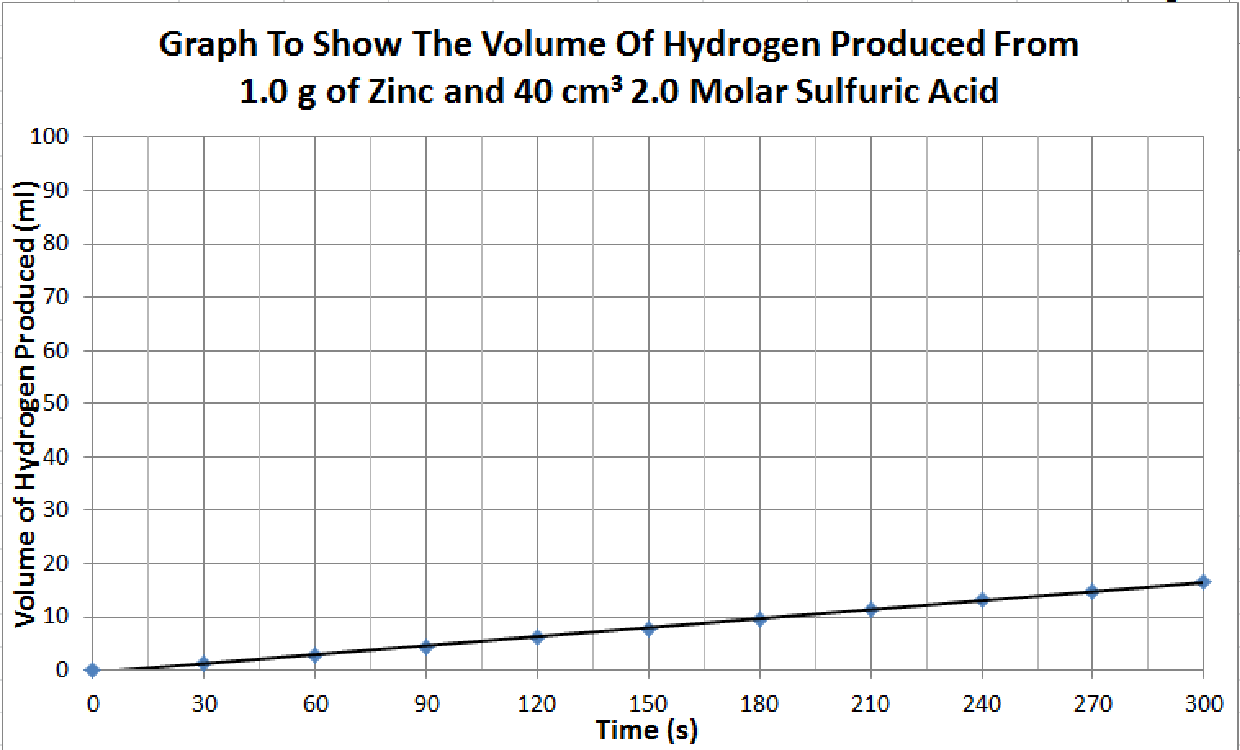
\includegraphics[width=\textwidth]{./Analysis/Images/1NonCatalyst/2Molar.pdf}
    \caption{2.0 Molar Sulfuric Acid and 1.0 g of Zinc Average Graph} \label{fig:2MolarSAGradient}
\end{figure}

$Gradient = \frac{16.67}{300}$

Therefore:

$Rate = 0.056 mol dm^{-3} s^{-1}$

\begin{figure}[H]
    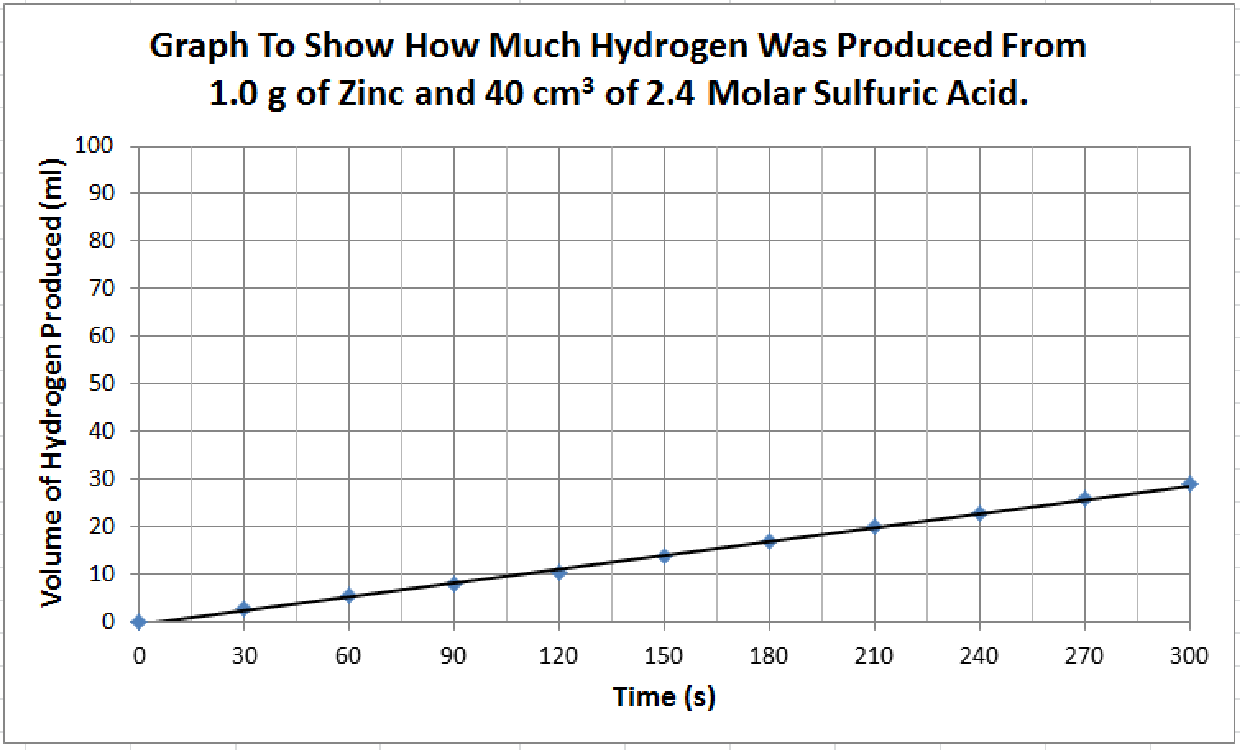
\includegraphics[width=\textwidth]{./Analysis/Images/1NonCatalyst/24Molar.pdf}
    \caption{2.4 Molar Sulfuric Acid and 1.0 g of Zinc Average Graph} \label{fig:24MolarSAGradient}
\end{figure}

$Gradient = \frac{28.83}{300}$

Therefore:

$Rate = 0.096 mol dm^{-3} s^{-1}$

\begin{figure}[H]
    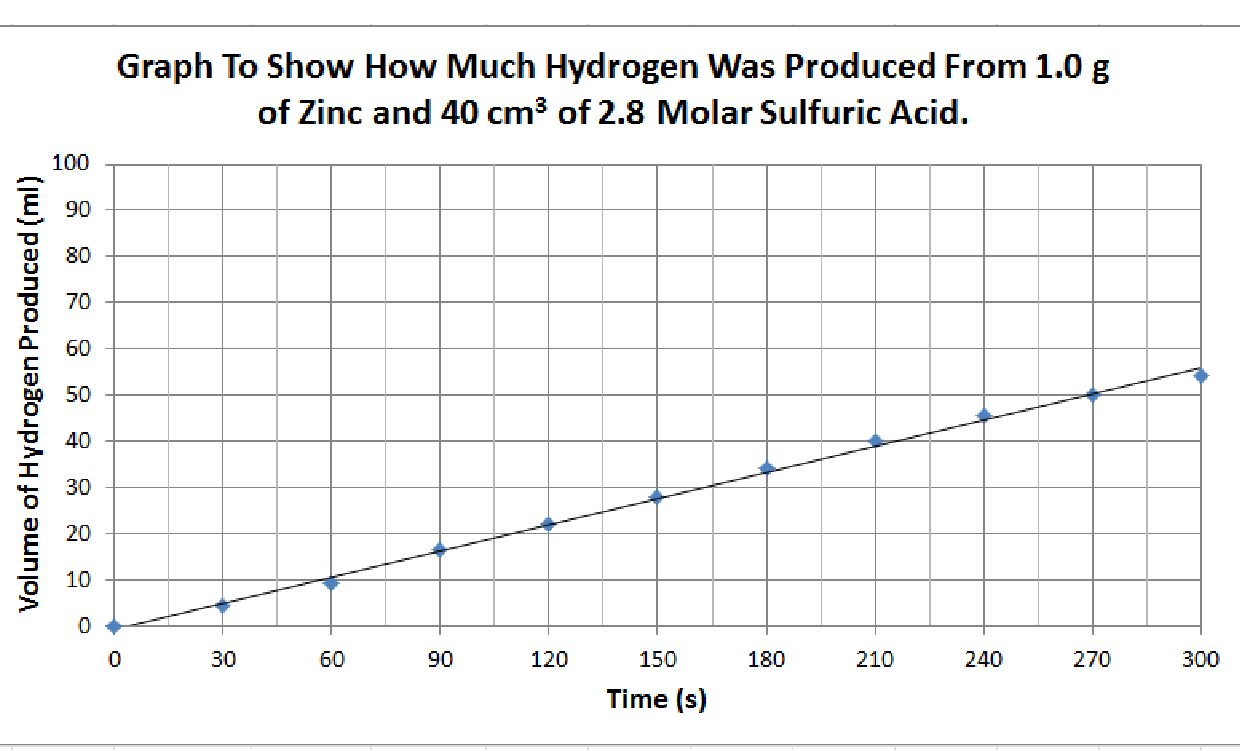
\includegraphics[width=\textwidth]{./Analysis/Images/1NonCatalyst/28Molar.pdf}
    \caption{2.8 Molar Sulfuric Acid and 1.0 g of Zinc Average Graph} \label{fig:28MolarSAGradient}
\end{figure}

$Gradient = \frac{55.50}{300}$

Therefore:

$Rate = 0.185 mol dm^{-3} s^{-1}$

\begin{figure}[H]
    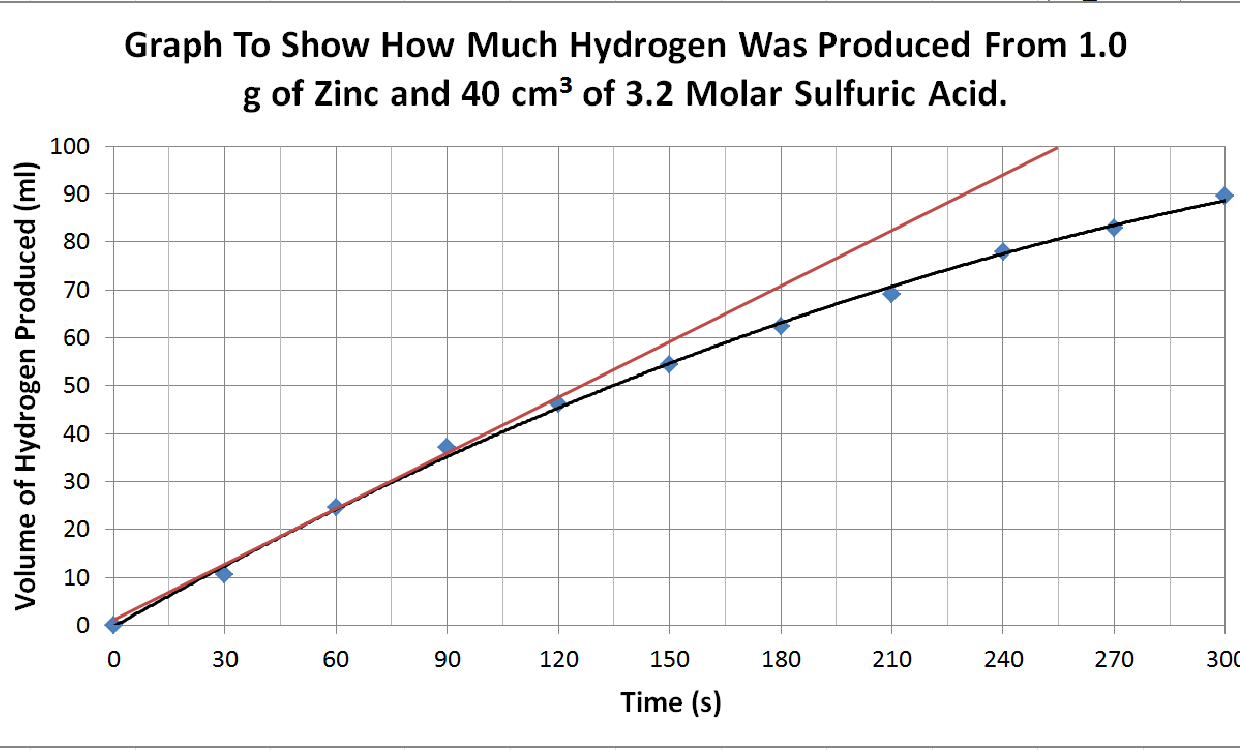
\includegraphics[width=\textwidth]{./Analysis/Images/1NonCatalyst/32Molar.pdf}
    \caption{3.2 Molar Sulfuric Acid and 1.0 g of Zinc Average Graph} \label{fig:32MolarSAGradient}
\end{figure}

$Gradient = \frac{100}{227.14}$

Therefore:

$Rate = 0.440 mol dm^{-3} s^{-1}$

\begin{figure}[H]
    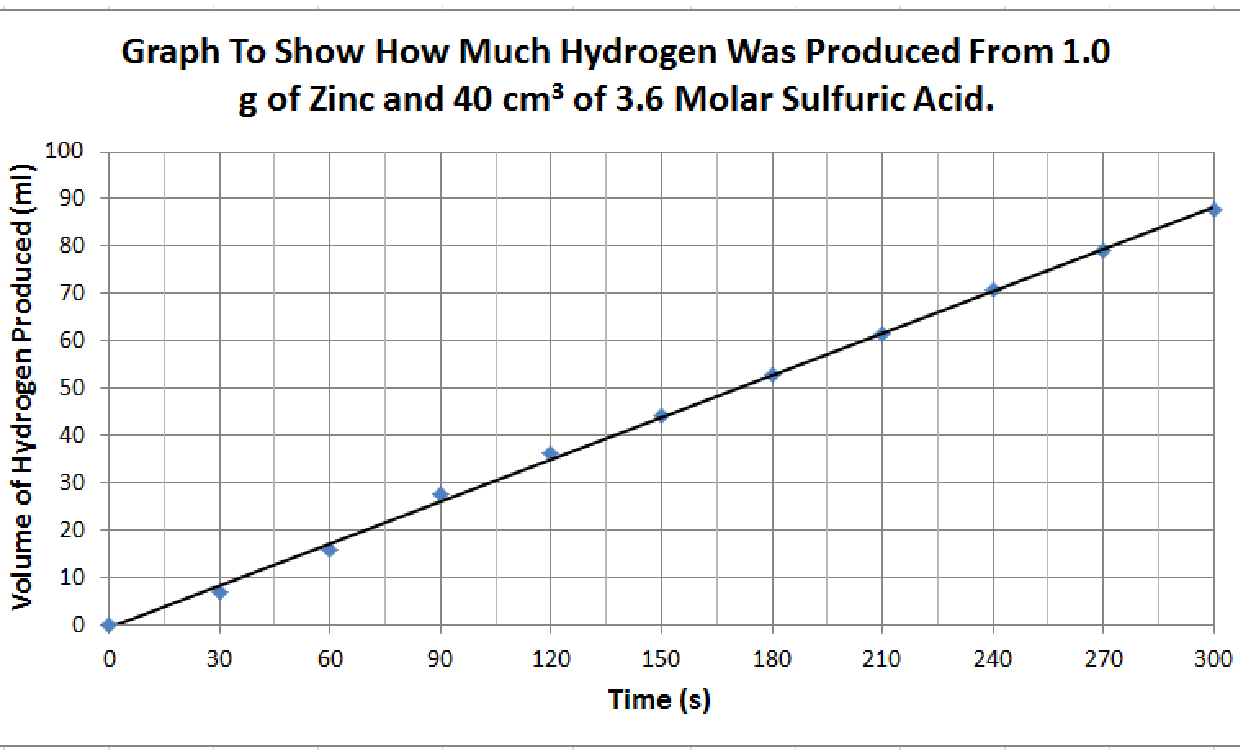
\includegraphics[width=\textwidth]{./Analysis/Images/1NonCatalyst/36Molar.pdf}
    \caption{3.6 Molar Sulfuric Acid and 1.0 g of Zinc Average Graph} \label{fig:36MolarSAGradient}
\end{figure}

$Gradient = \frac{87.67}{300}$

Therefore:

$Rate = 0.292 mol dm^{-3} s^{-1}$

\begin{figure}[H]
    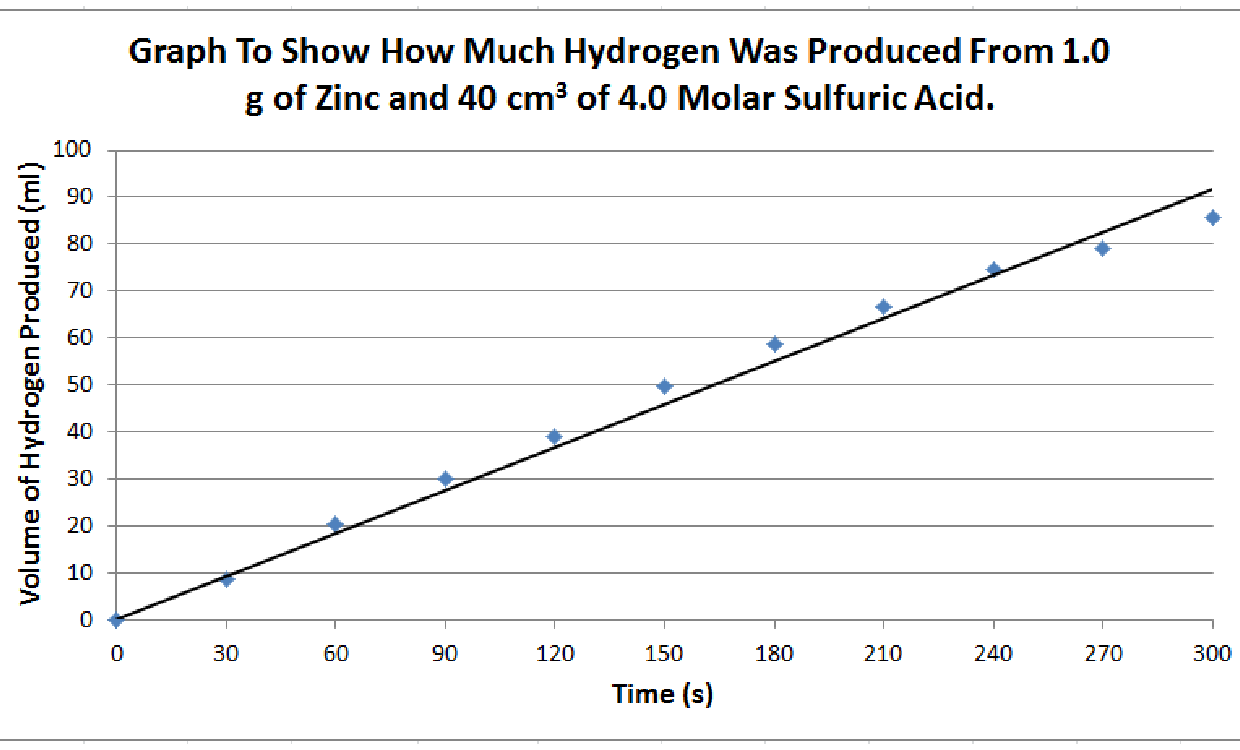
\includegraphics[width=\textwidth]{./Analysis/Images/1NonCatalyst/40Molar.pdf}
    \caption{4.0 Molar Sulfuric Acid and 1.0 g of Zinc Average Graph} \label{fig:40MolarSAGradient}
\end{figure}

$Gradient = \frac{92}{300}$

Therefore:

$Rate = 0.307 mol dm^{-3} s^{-1}$

Below the rates of reactions are summarised in a table.

\begin{figure}[H]
    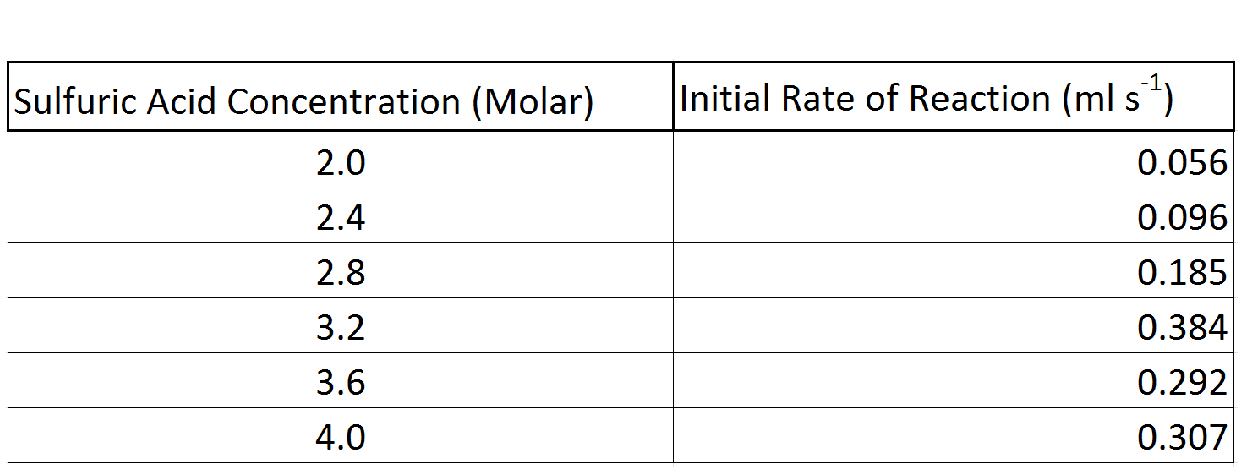
\includegraphics[width=\textwidth]{./Analysis/Images/1NonCatalyst/Rates.pdf}
    \caption{Initial Rates of Reactions for the Non-Catalysed Zinc and Sulfuric Acid Reaction} \label{fig:RatesSA}
\end{figure}

Below the rates of reactions are compiled into a progress graph.

\begin{figure}[H]
    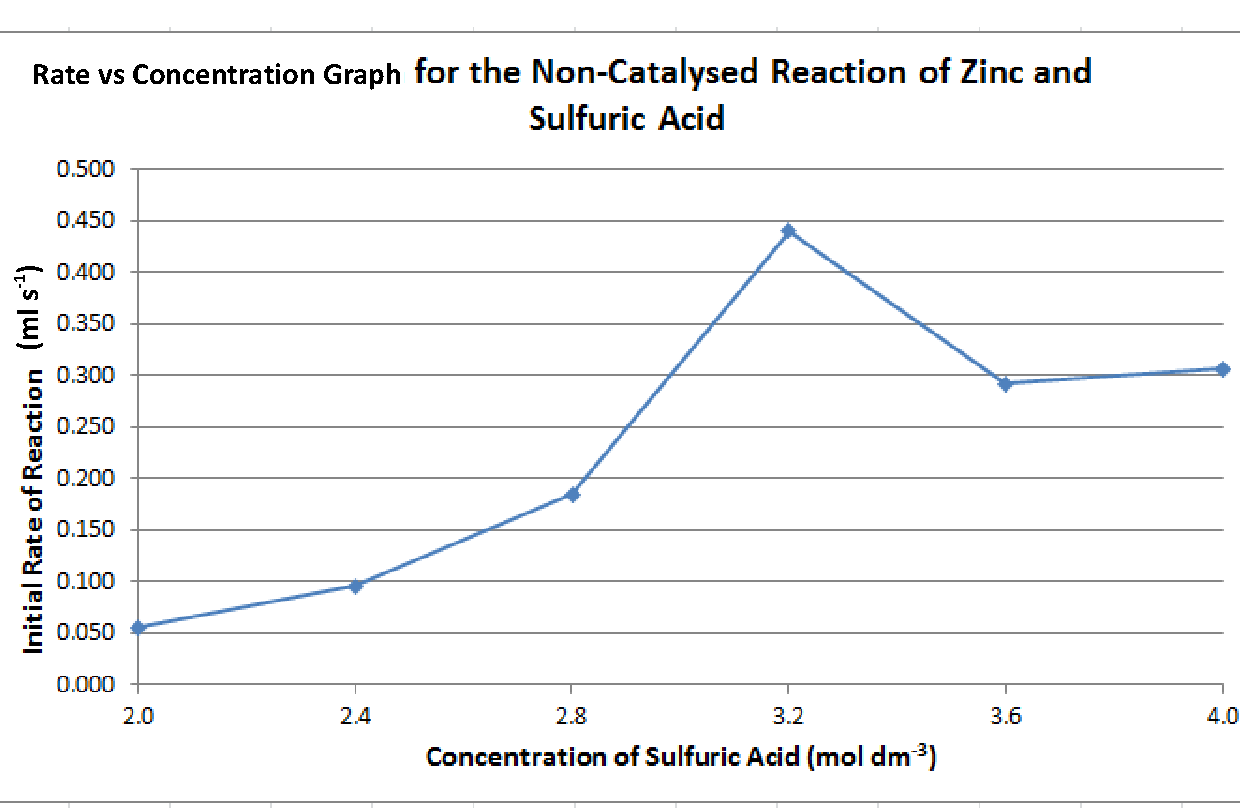
\includegraphics[width=\textwidth]{./Analysis/Images/1NonCatalyst/ProgressGraph.pdf}
    \caption{Progress Graph for the Non-Catalysed Reaction} \label{fig:ProgressGraphSA}
\end{figure}

The progress graph for this experiment appears to be a second order reaction up to 3.2 Molar; however I believe that the zinc clumps at higher concentrations of acids, which would explain the decreased rate of reaction after 3.2 molar. Therefore I think that the order of sulfuric acid without the presence of a catalyst is second order. This means that doubling the concentration of sulfuric acid in this reaction quadruples the initial rate of reaction. The rate equation for this reaction would be:

$Rate = k [Sulfuric Acid]$

In order to work out the rate constant of this equation, the equation has to be re-arranged to:

$k = \frac{Rate}{[Sulfuric Acid]^2}$

By putting my experimental result from the 2.8 molar concentration series into the equation you get:

$k = \frac{0.185}{2.8^2}$

Therefore the rate constant 'k' is equal to 0.0236 to 3 significant figures.



\section{Zinc and Sulfuric Acid With a Copper Sulfate Catalyst}


	\subsection{Sulfuric Acid}

Below are the graphs that I have used to work out the rate of the reaction for the experiment series that did involve a catalyst but varied in sulfuric acid concentration. All graphs have taken a mean average of the three repeats in order to plot the data points. As discussed in my 'Chosen Method' section on page \pageref{Chosen Method} I am using the equation $Gradient = \frac{Change in Y}{Change in X}$ and as the gradient is equal to the rate of reaction, I will be able to use the graphs below in order to generate a progress graph which will determine the order of the reaction. I will calculate all rates to 3 decimal places.


\begin{figure}[H]
    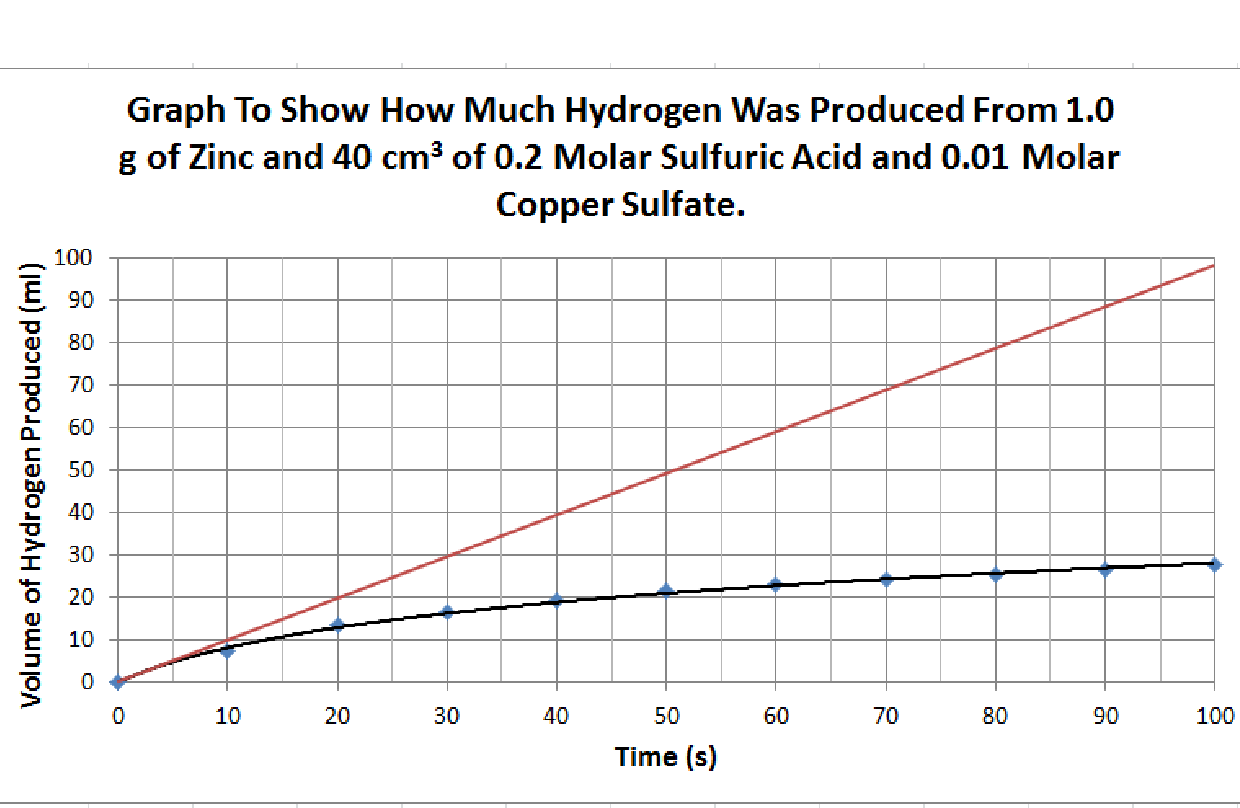
\includegraphics[width=\textwidth]{./Analysis/Images/2Catalysed/02Molar.pdf}
    \caption{0.2 Molar Sulfuric Acid and 0.01 Molar Copper Sulfate and 1.0 g of Zinc Average Graph} \label{fig:02MolarSACSGradient}
\end{figure}

$Gradient = \frac{97}{100}$

Therefore:

$Rate = 0.970 mol dm^{-3} s^{-1}$

\begin{figure}[H]
    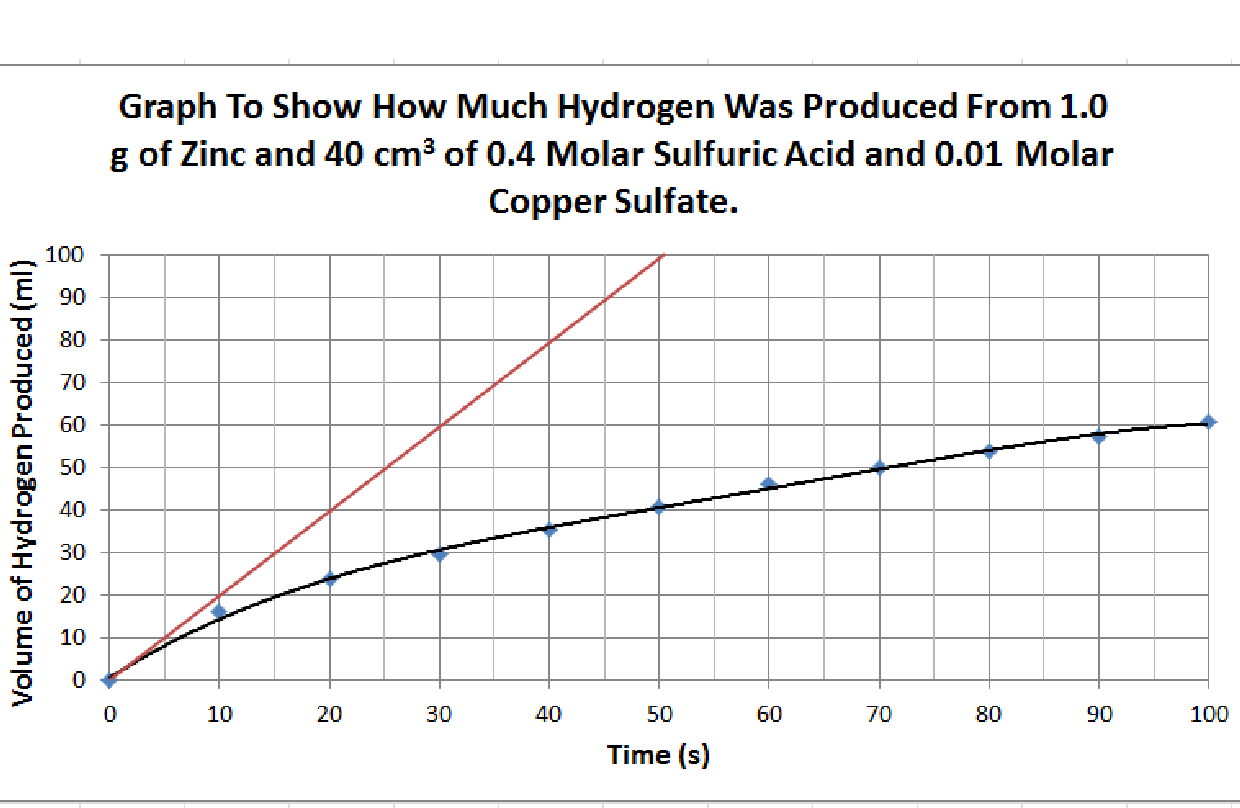
\includegraphics[width=\textwidth]{./Analysis/Images/2Catalysed/04Molar.pdf}
    \caption{0.4 Molar Sulfuric Acid and 0.01 Molar Copper Sulfate and 1.0 g of Zinc Average Graph} \label{fig:04MolarSACSGradient}
\end{figure}

$Gradient = \frac{100}{51.5}$

Therefore:

$Rate = 1.942 mol dm^{-3} s^{-1}$

\begin{figure}[H]
    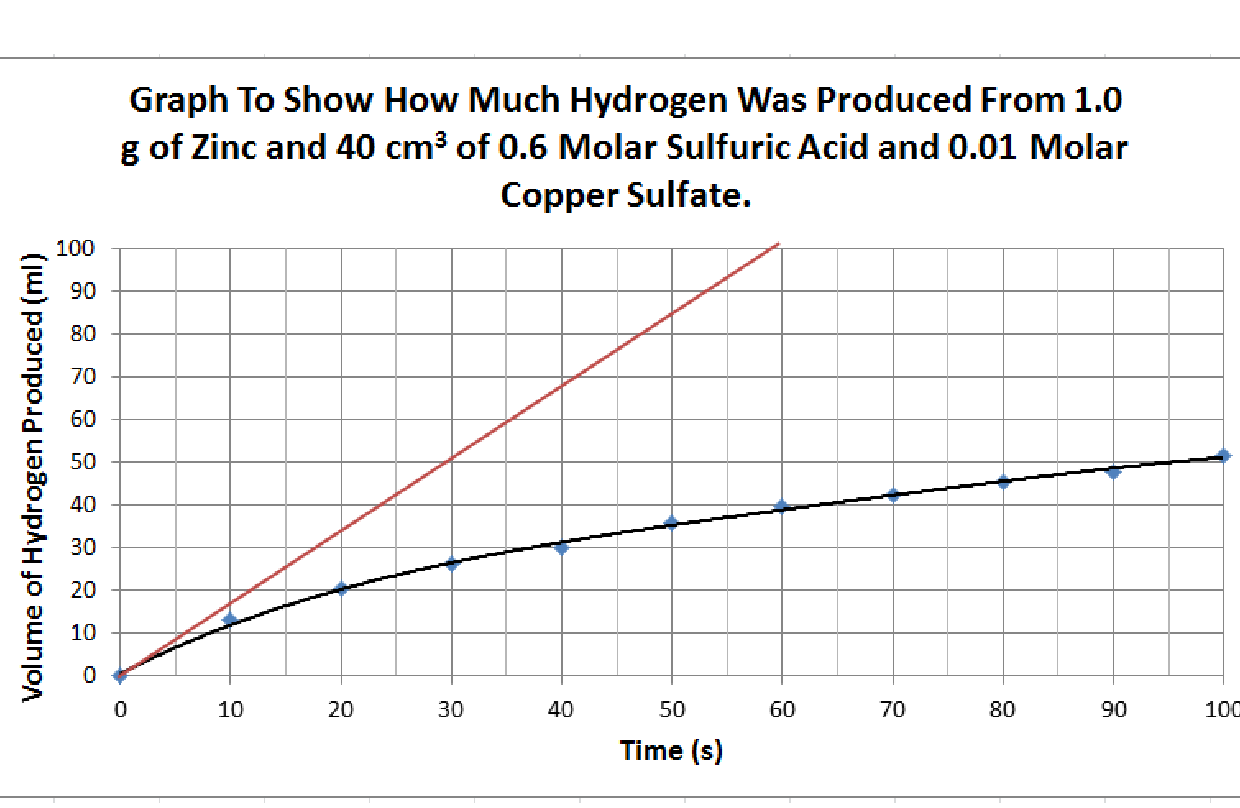
\includegraphics[width=\textwidth]{./Analysis/Images/2Catalysed/06Molar.pdf}
    \caption{0.6 Molar Sulfuric Acid and 0.01 Molar Copper Sulfate and 1.0 g of Zinc Average Graph} \label{fig:06MolarSACSGradient}
\end{figure}

$Gradient = \frac{100}{59}$

Therefore:

$Rate = 1.695 mol dm^{-3} s^{-1}$

\begin{figure}[H]
    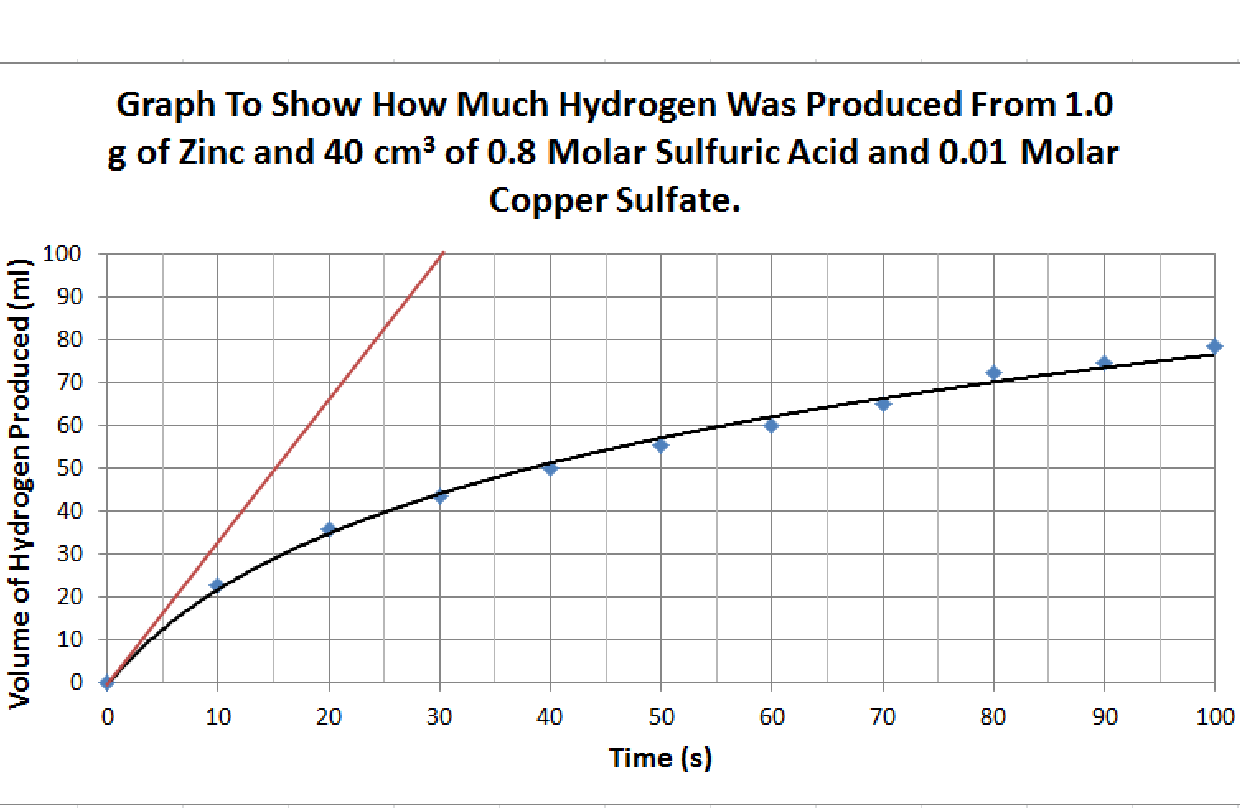
\includegraphics[width=\textwidth]{./Analysis/Images/2Catalysed/08Molar.pdf}
    \caption{0.8 Molar Sulfuric Acid and 0.01 Molar Copper Sulfate and 1.0 g of Zinc Average Graph} \label{fig:08MolarSACSGradient}
\end{figure}

$Gradient = \frac{100}{30.7}$

Therefore:

$Rate = 3.257 mol dm^{-3} s^{-1}$

\begin{figure}[H]
    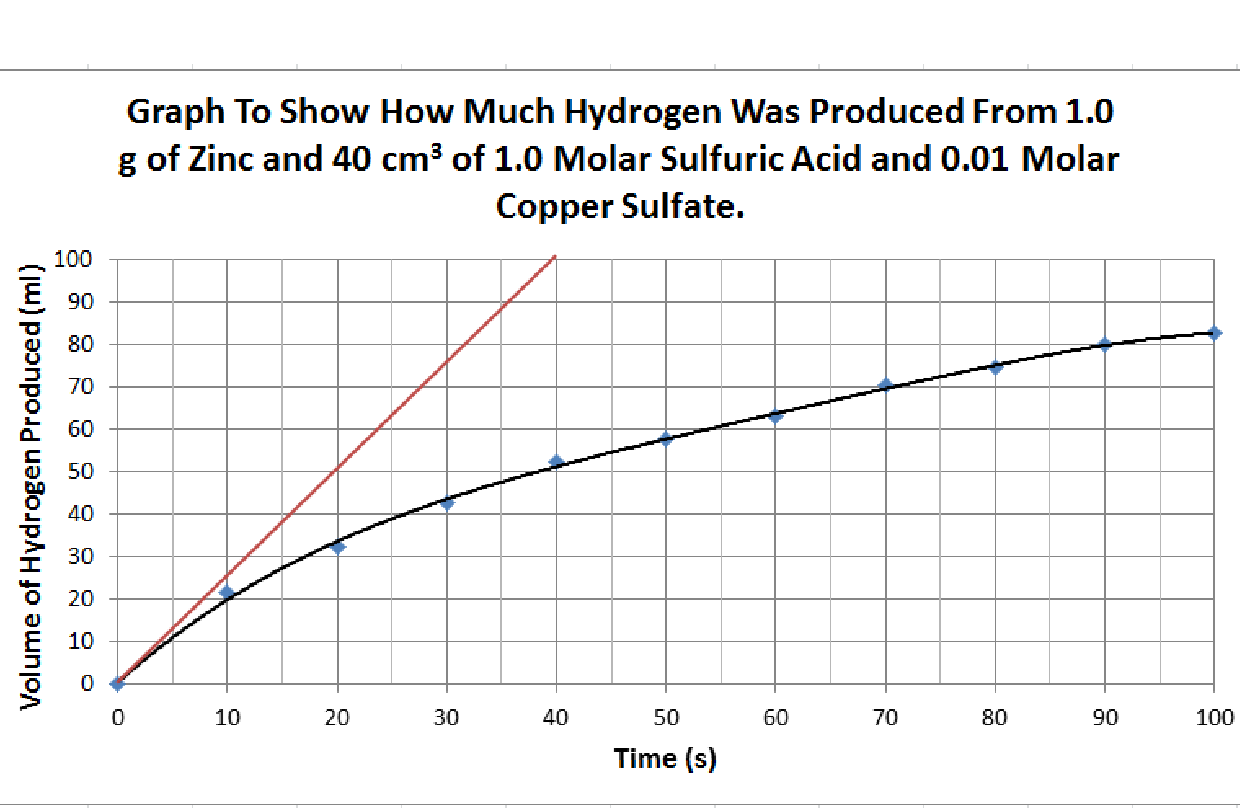
\includegraphics[width=\textwidth]{./Analysis/Images/2Catalysed/10Molar.pdf}
    \caption{1.0 Molar Sulfuric Acid and 0.01 Molar Copper Sulfate and 1.0 g of Zinc Average Graph} \label{fig:10MolarSACSGradient}
\end{figure}

$Gradient = \frac{100}{40}$

Therefore:

$Rate = 2.500 mol dm^{-3} s^{-1}$

\begin{figure}[H]
    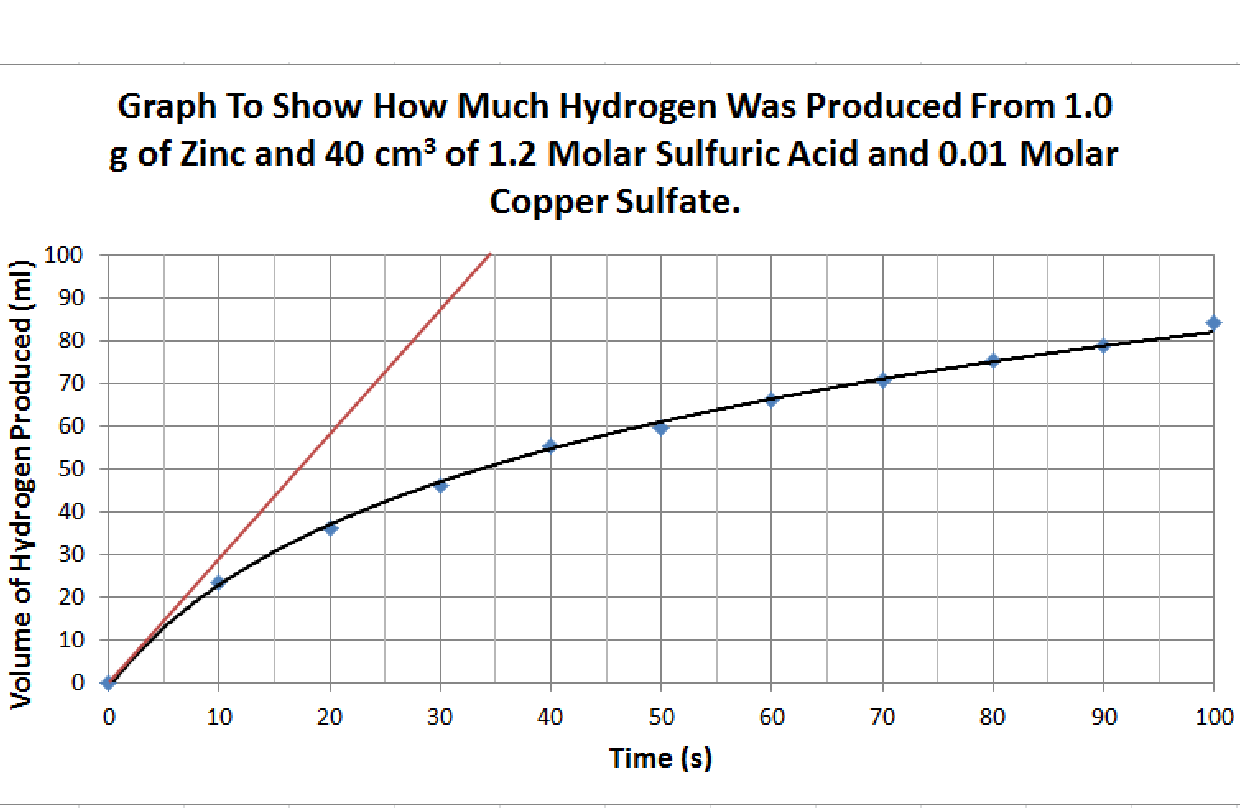
\includegraphics[width=\textwidth]{./Analysis/Images/2Catalysed/12Molar.pdf}
    \caption{1.2 Molar Sulfuric Acid and 0.01 Molar Copper Sulfate and 1.0 g of Zinc Average Graph} \label{fig:12MolarSACSGradient}
\end{figure}

$Gradient = \frac{100}{34.5}$

Therefore:

$Rate = 2.899 mol dm^{-3} s^{-1}$

Below the rates of reactions are summarised in a table.

\begin{figure}[H]
    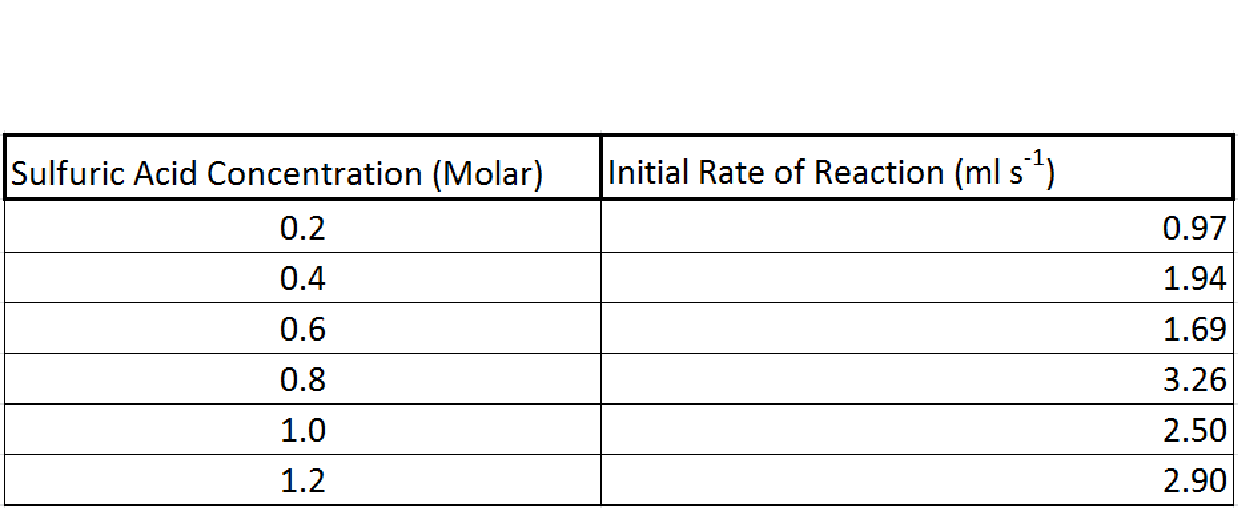
\includegraphics[width=\textwidth]{./Analysis/Images/2Catalysed/Rates.pdf}
    \caption{Initial Rates of Reactions for the Catalysed Zinc and Sulfuric Acid Reaction} \label{fig:RatesSACS}
\end{figure}

Below the rates of reactions are compiled into a progress graph.

\begin{figure}[H]
    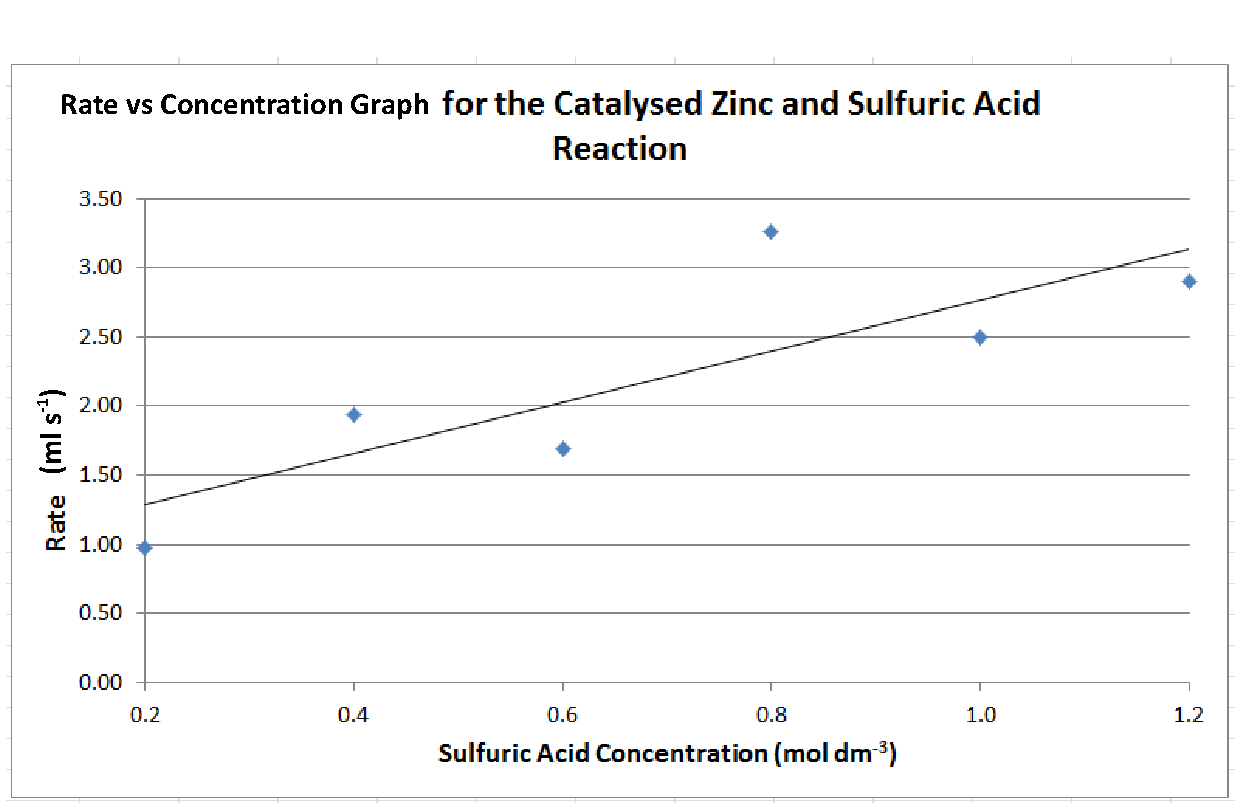
\includegraphics[width=\textwidth]{./Analysis/Images/2Catalysed/ProgressGraph.pdf}
    \caption{Progress Graph for the Catalysed Zinc and Sulfuric Acid Reaction} \label{fig:ProgressGraphSACS}
\end{figure}

The progress graph for this experiment is too scattered to get an accurate result; however due to the scattered result it appears that a straight line of best fit would be most appropriate. Therefore I believe that the when in the presence of copper sulfate, sulfuric acid is a first order reactant.This means that doubling the concentration of sulfuric acid in this reaction doubles the initial rate of reaction. The rate equation for this reaction would be:

$Rate = k [Sulfuric Acid]$

Next I will work out if copper sulfate is also part of the rate equation.

	\subsection{Copper Sulfate}
Below are the graphs that I have used to work out the rate of the reaction for the experiment series that did involve a catalyst and varied in copper sulfate concentration. All graphs have taken a mean average of the three repeats in order to plot the data points. As discussed in my 'Chosen Method' section on page \pageref{Chosen Method} I am using the equation $Gradient = \frac{Change in Y}{Change in X}$ and as the gradient is equal to the rate of reaction, I will be able to use the graphs below in order to generate a progress graph which will determine the order of the reaction. I will calculate all rates to 3 decimal places.


\begin{figure}[H]
    \includegraphics[width=\textwidth]{./Analysis/Images/3VaryCopperSulfate/001Molar.pdf}
    \caption{0.4 Molar Sulfuric Acid and 0.01 Molar Copper Sulfate and 1.0 g of Zinc Average Graph} \label{fig:001VaryCopperSulfate}
\end{figure}

$Gradient = \frac{70}{58}$

Therefore:

$Rate = 1.207 mol dm^{-3} s^{-1}$

\begin{figure}[H]
    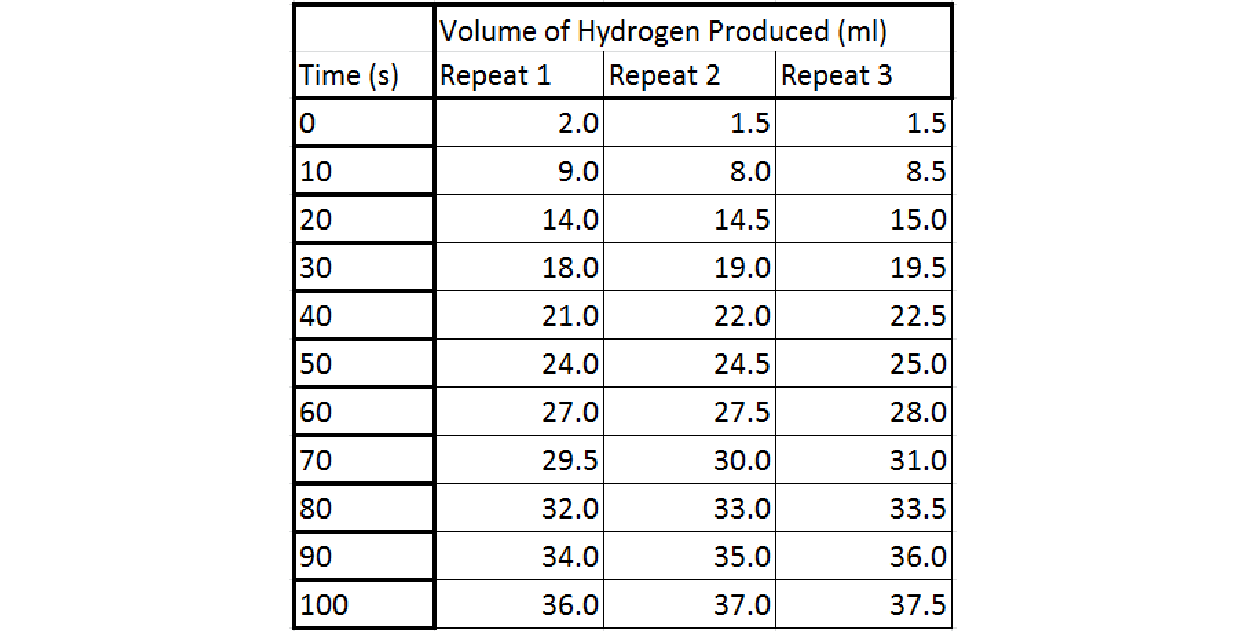
\includegraphics[width=\textwidth]{./Analysis/Images/3VaryCopperSulfate/002Molar.pdf}
    \caption{0.4 Molar Sulfuric Acid and 0.02 Molar Copper Sulfate and 1.0 g of Zinc Average Graph} \label{fig:002VaryCopperSulfate}
\end{figure}

$Gradient = \frac{79}{90}$

Therefore:

$Rate = 0.778 mol dm^{-3} s^{-1}$

\begin{figure}[H]
    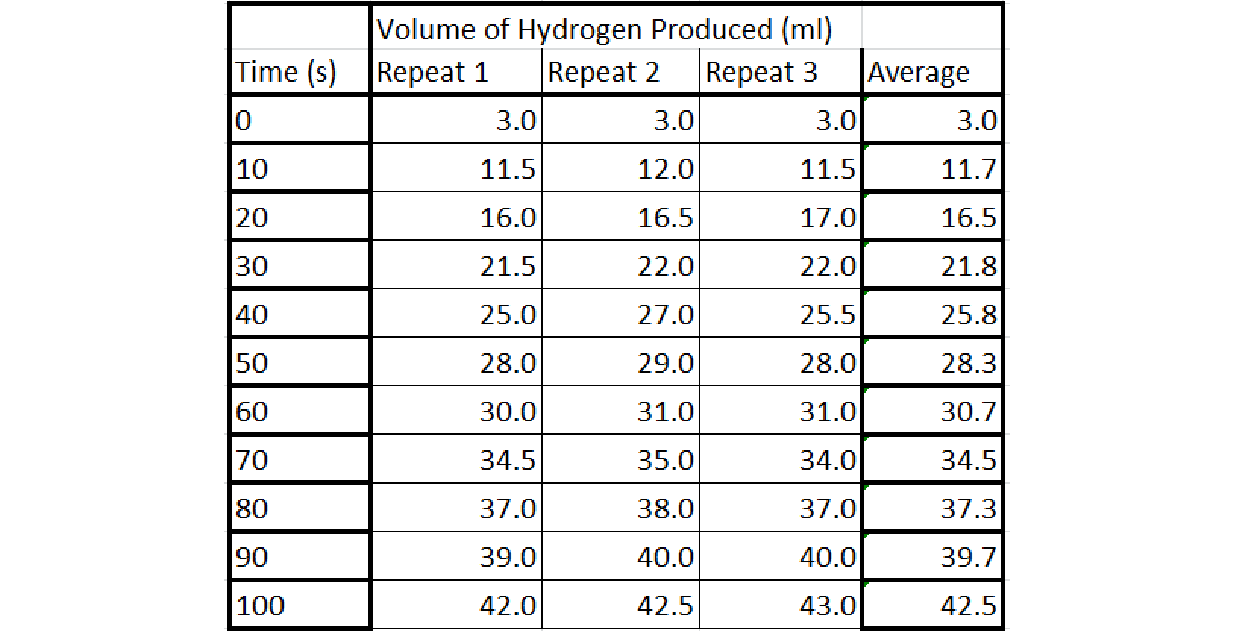
\includegraphics[width=\textwidth]{./Analysis/Images/3VaryCopperSulfate/003Molar.pdf}
    \caption{0.4 Molar Sulfuric Acid and 0.03 Molar Copper Sulfate and 1.0 g of Zinc Average Graph} \label{fig:003VaryCopperSulfate}
\end{figure}

$Gradient = \frac{70}{60}$

Therefore:

$Rate = 1.167 mol dm^{-3} s^{-1}$

\begin{figure}[H]
    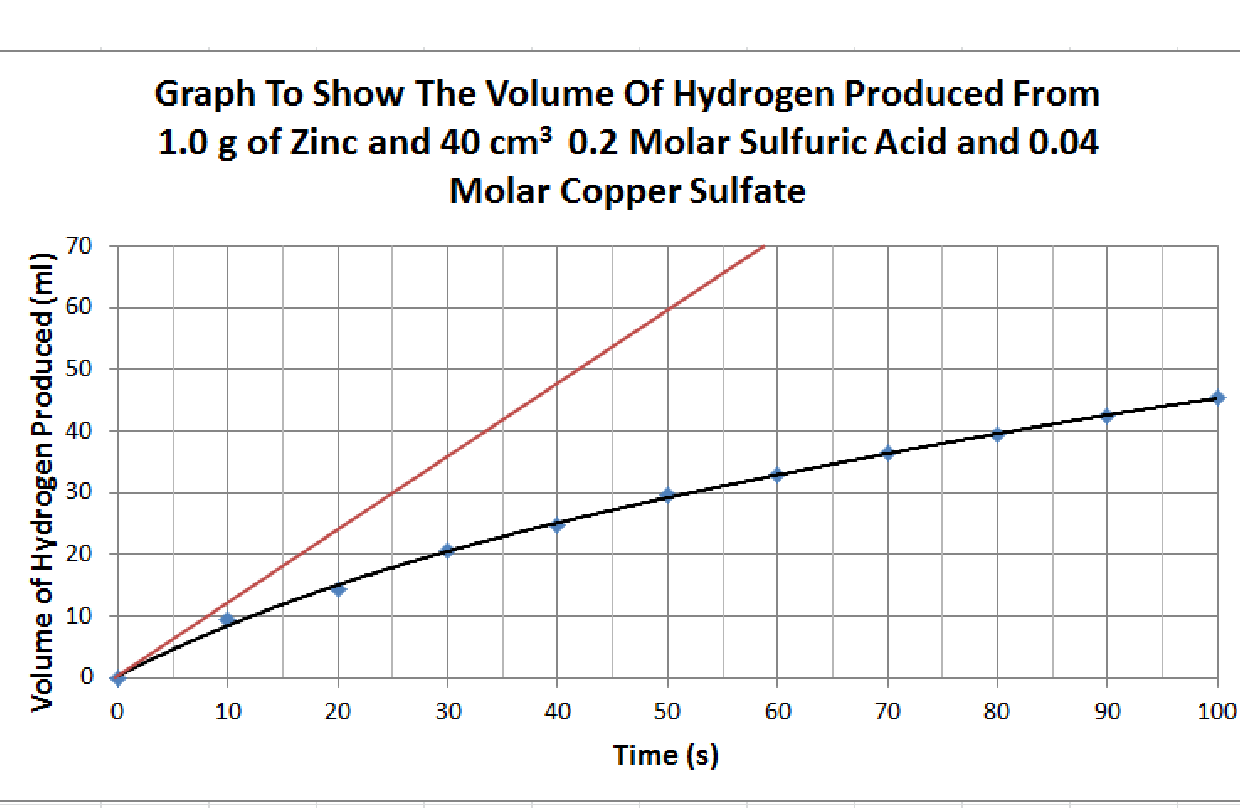
\includegraphics[width=\textwidth]{./Analysis/Images/3VaryCopperSulfate/004Molar.pdf}
    \caption{0.4 Molar Sulfuric Acid and 0.04 Molar Copper Sulfate and 1.0 g of Zinc Average Graph} \label{fig:004VaryCopperSulfate}
\end{figure}

$Gradient = \frac{70}{57.5}$

Therefore:

$Rate = 1.217 mol dm^{-3} s^{-1}$

\begin{figure}[H]
    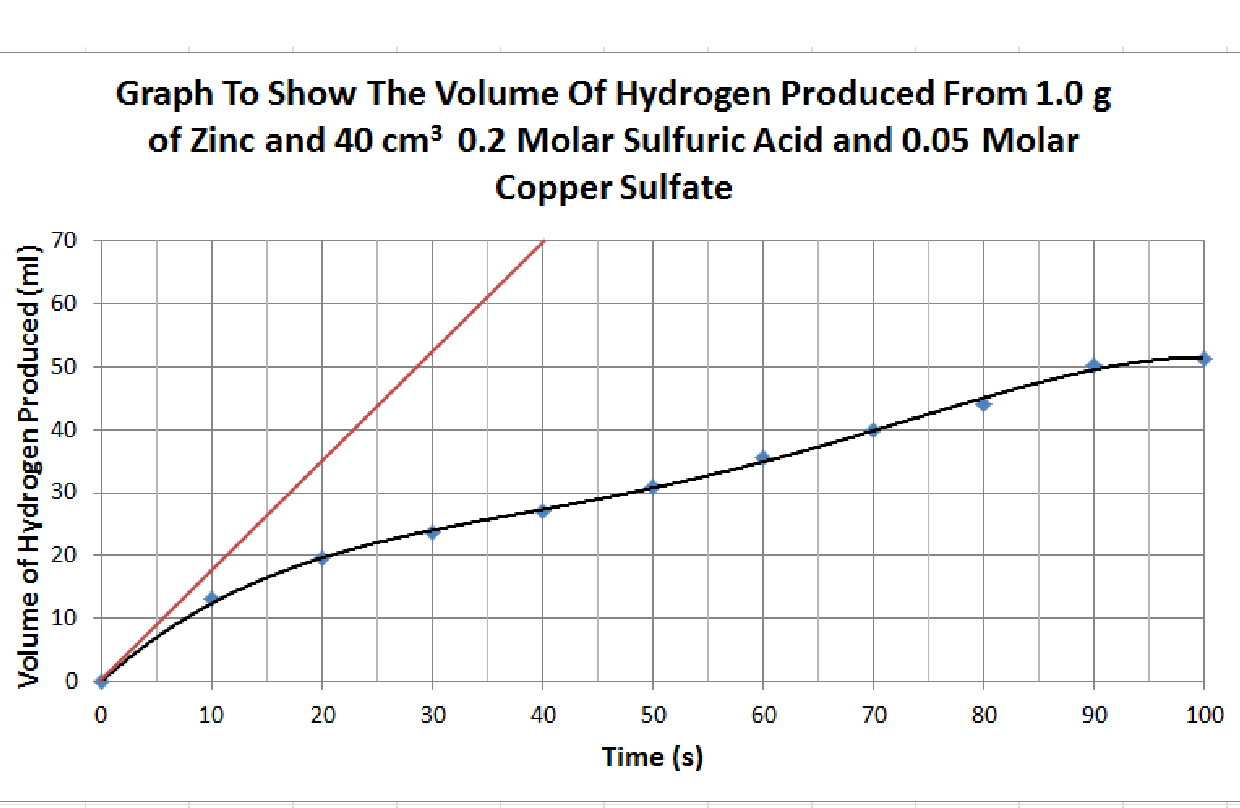
\includegraphics[width=\textwidth]{./Analysis/Images/3VaryCopperSulfate/005Molar.pdf}
    \caption{0.4 Molar Sulfuric Acid and 0.05 Molar Copper Sulfate and 1.0 g of Zinc Average Graph} \label{fig:005VaryCopperSulfate}
\end{figure}

$Gradient = \frac{70}{40}$

Therefore:

$Rate = 1.750 mol dm^{-3} s^{-1}$

\begin{figure}[H]
    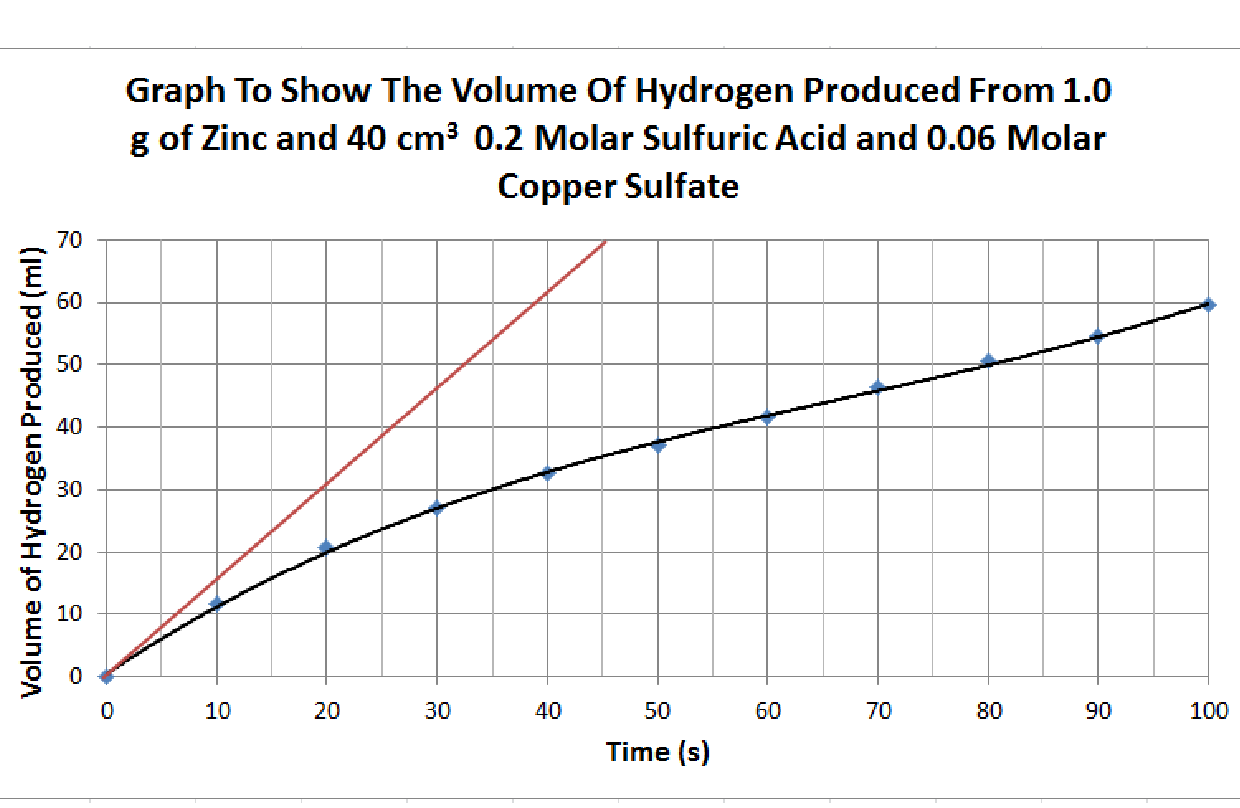
\includegraphics[width=\textwidth]{./Analysis/Images/3VaryCopperSulfate/006Molar.pdf}
    \caption{0.4 Molar Sulfuric Acid and 0.06 Molar Copper Sulfate and 1.0 g of Zinc Average Graph} \label{fig:006VaryCopperSulfate}
\end{figure}
$Gradient = \frac{70}{45}$

Therefore:

$Rate = 1.556 mol dm^{-3} s^{-1}$

Below the rates of reactions are summarised in a table.

\begin{figure}[H]
    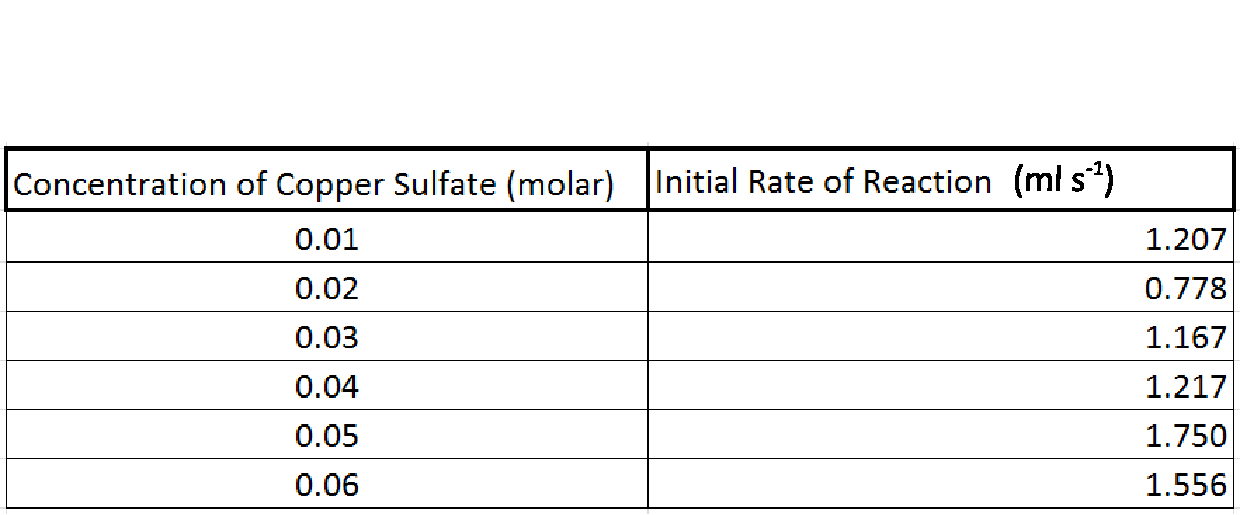
\includegraphics[width=\textwidth]{./Analysis/Images/3VaryCopperSulfate/Rates.pdf}
    \caption{Initial Rates of Reactions for the Catalysed Zinc and Sulfuric Acid Reaction} \label{fig:RatesSACSVary}
\end{figure}

Below the rates of reactions are compiled into a progress graph.

\begin{figure}[H]
    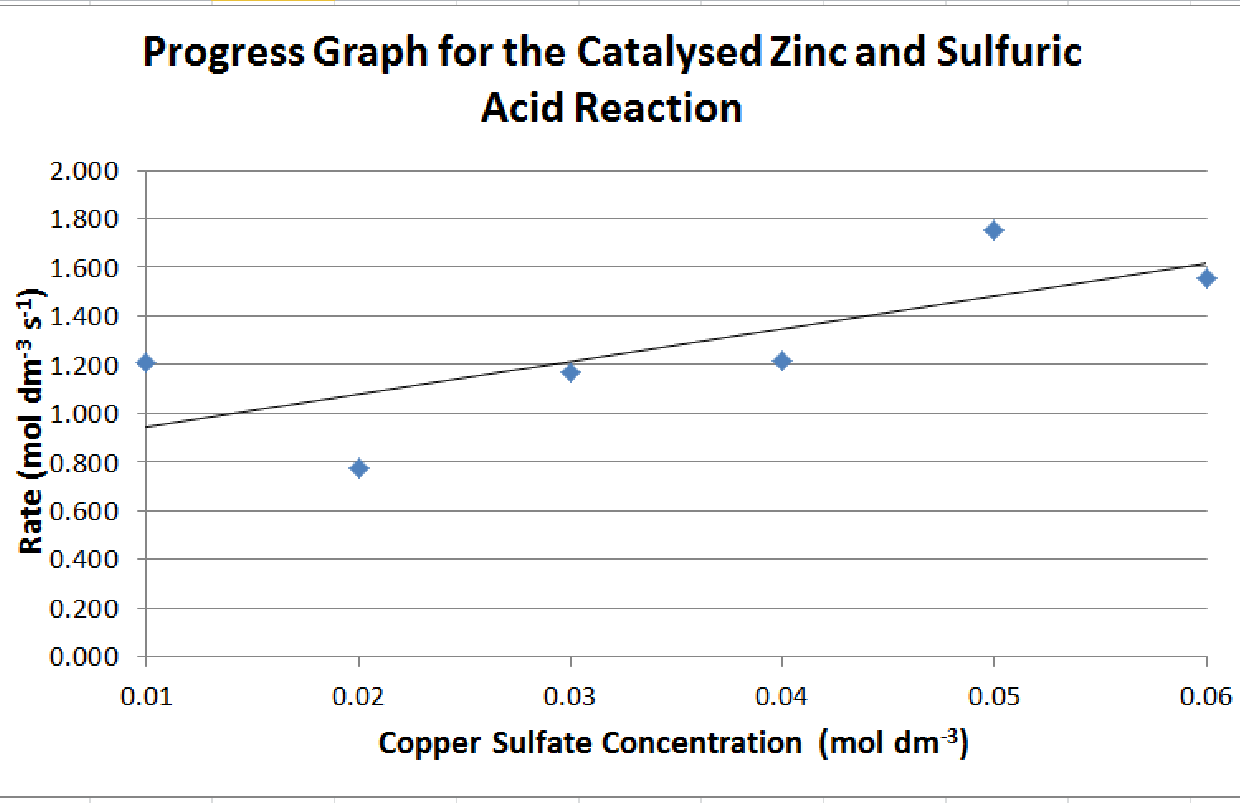
\includegraphics[width=\textwidth]{./Analysis/Images/3VaryCopperSulfate/ProgressGraph.pdf}
    \caption{Progress Graph for the Catalysed Zinc and Sulfuric Acid Reaction} \label{fig:ProgressGraphSACSVary}
\end{figure}

The progress graph for this experiment, again,  is too scattered to get an accurate result; however due to the scattered result it appears that a straight line of best fit would be most appropriate. Therefore I believe that the copper sulfate is a first order reactant. This means that doubling the concentration of copper sulfate in this reaction doubles the initial rate of reaction. The rate equation for this overall reaction would be:

$Rate = k [Sulfuric Acid] [Copper Sulfate]$

This means that overall the reaction is a second order reaction and both individual reactants are first order reactants.





\section{Comparing Catalysts}

The copper sulfate graph can be found on page \pageref{fig:04MolarSACSGradient}, Figure \ref{fig:04MolarSACSGradient}.

\begin{figure}[H]
    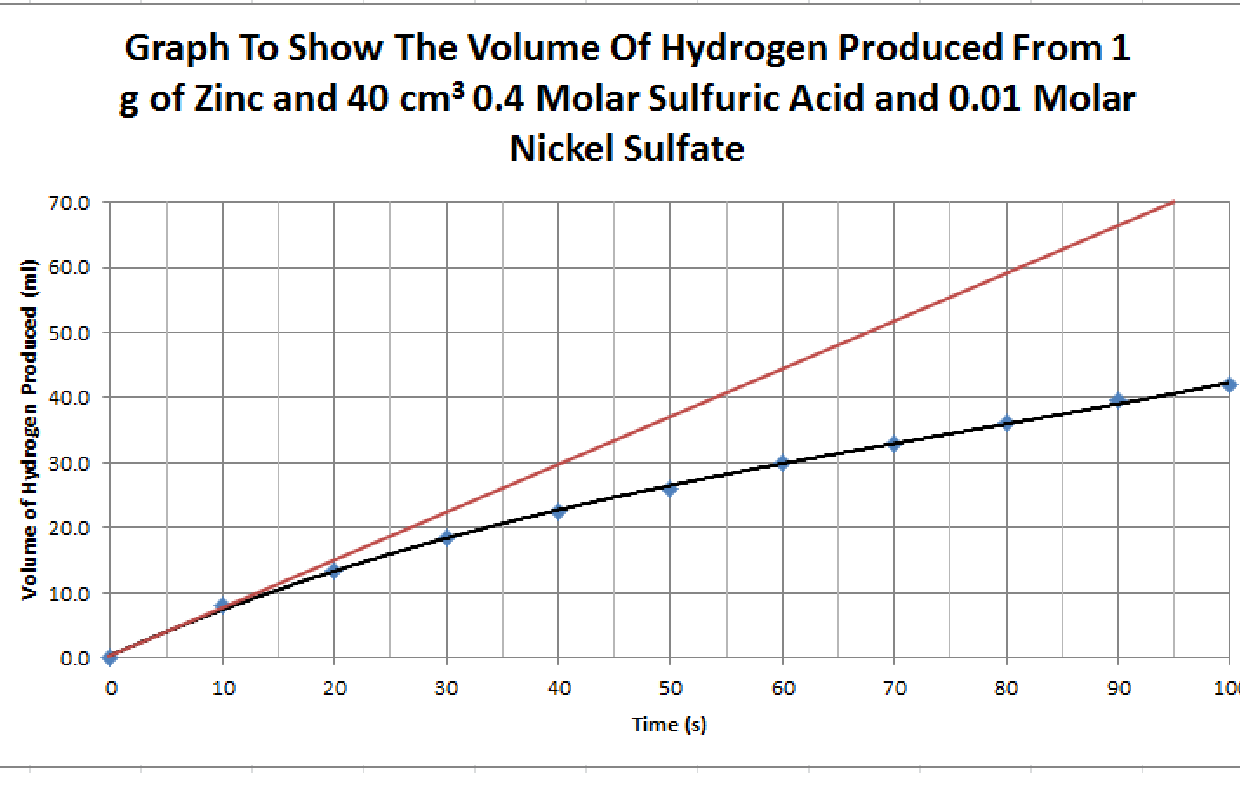
\includegraphics[width=\textwidth]{./Analysis/Images/4DifferentCatalysts/Nickel.pdf}
    \caption{0.4 Molar Sulfuric Acid and 0.01 Molar Nickel Sulfate and 1.0 g of Zinc Average Graph} \label{fig:NickelGradient}
\end{figure}

\begin{figure}[H]
    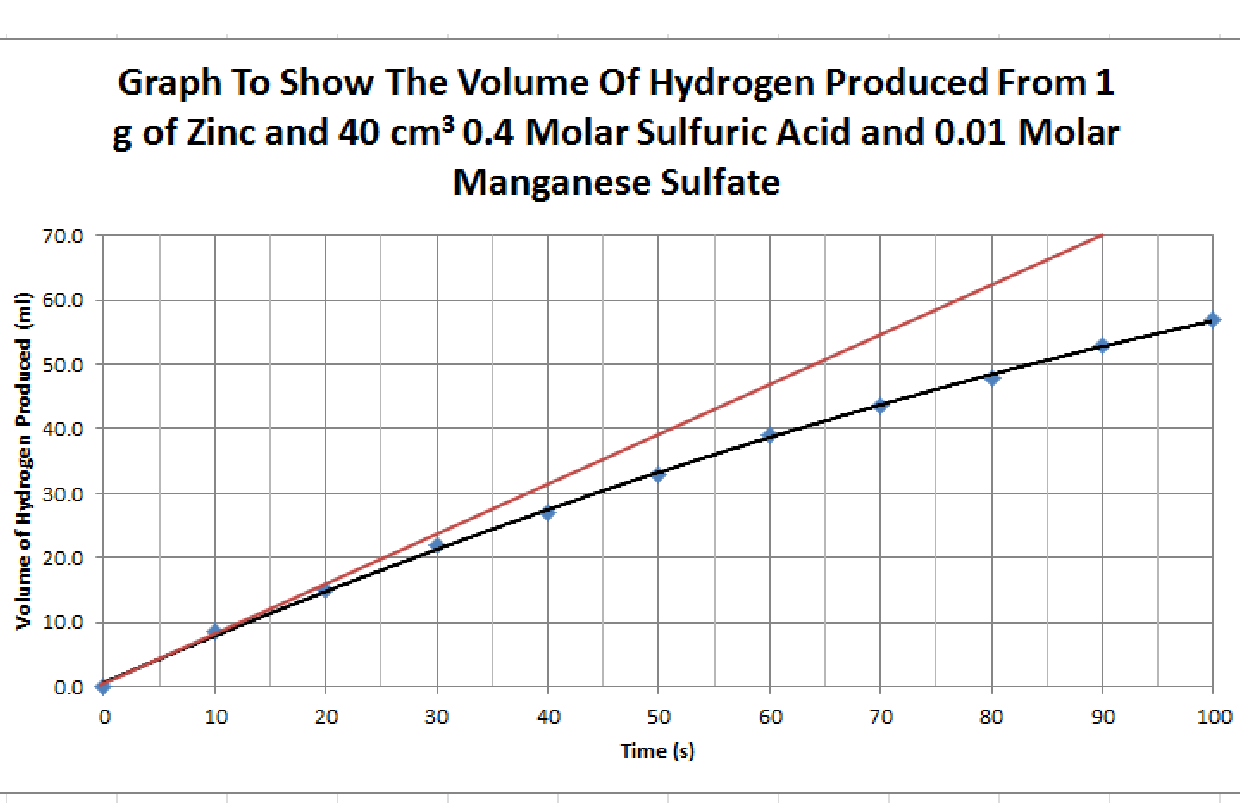
\includegraphics[width=\textwidth]{./Analysis/Images/4DifferentCatalysts/Manganese.pdf}
    \caption{0.4 Molar Sulfuric Acid and 0.01 Molar Manganese Sulfate and 1.0 g of Zinc Average Graph} \label{fig:ManganeseGradient}
\end{figure}

\begin{figure}[H]
    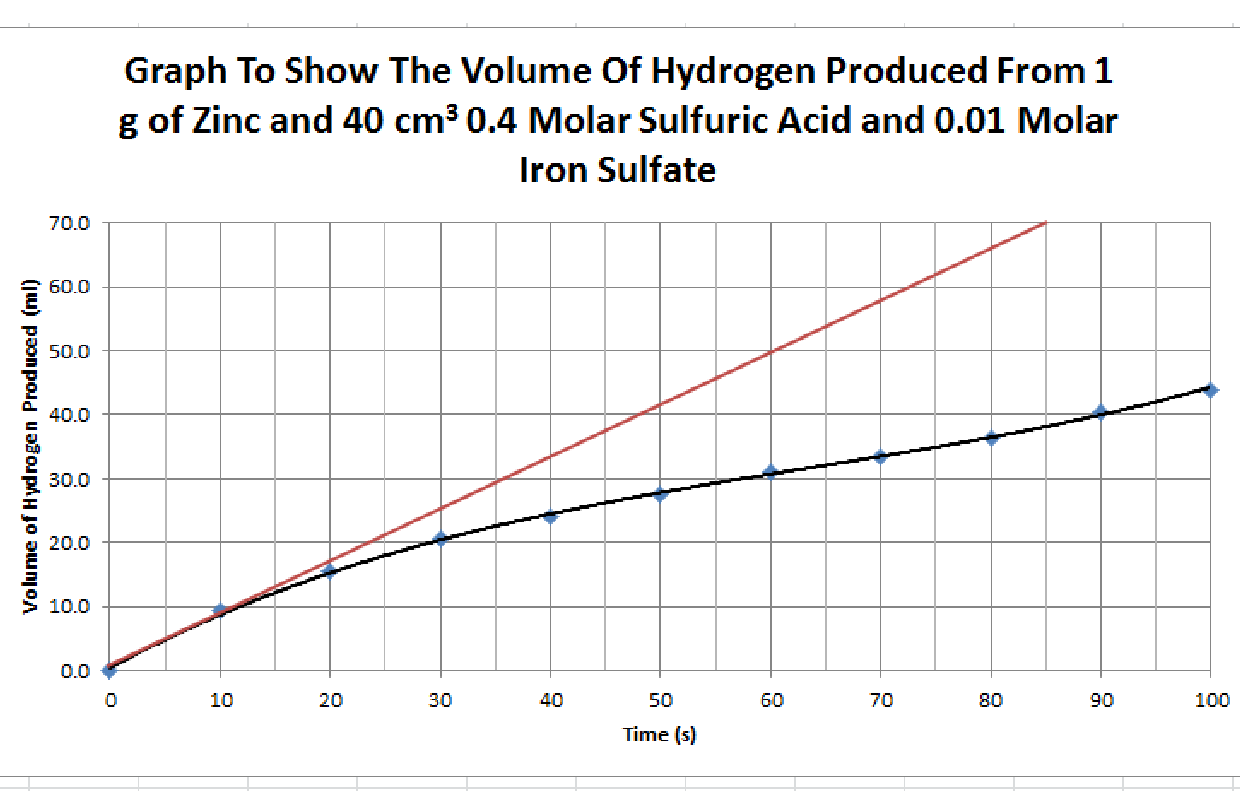
\includegraphics[width=\textwidth]{./Analysis/Images/4DifferentCatalysts/Iron.pdf}
    \caption{0.4 Molar Sulfuric Acid and 0.01 Molar Iron Sulfate and 1.0 g of Zinc Average Graph} \label{fig:IronGradient}
\end{figure}

Below the rates of reactions are summarised in a table.

\begin{figure}[H]
    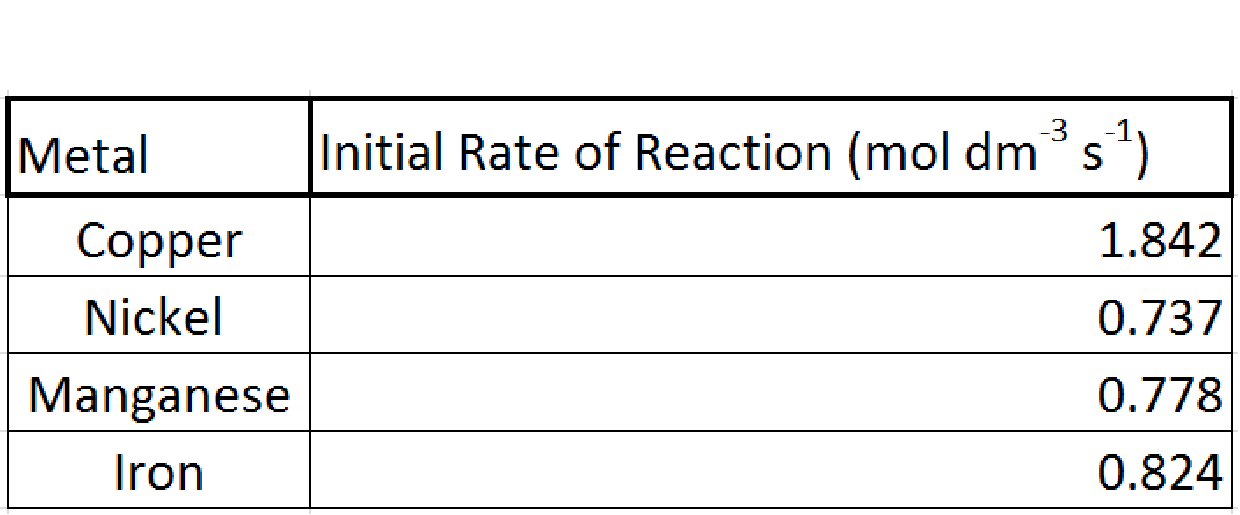
\includegraphics[width=\textwidth]{./Analysis/Images/4DifferentCatalysts/Rates.pdf}
    \caption{Initial Rates of Reactions for the Different Catalysts Tested} \label{fig:RatesDiffCat}
\end{figure}


 For this experiment I have created a bar chart to compare the rate of reaction, this can be seen below.

\begin{figure}[H]
    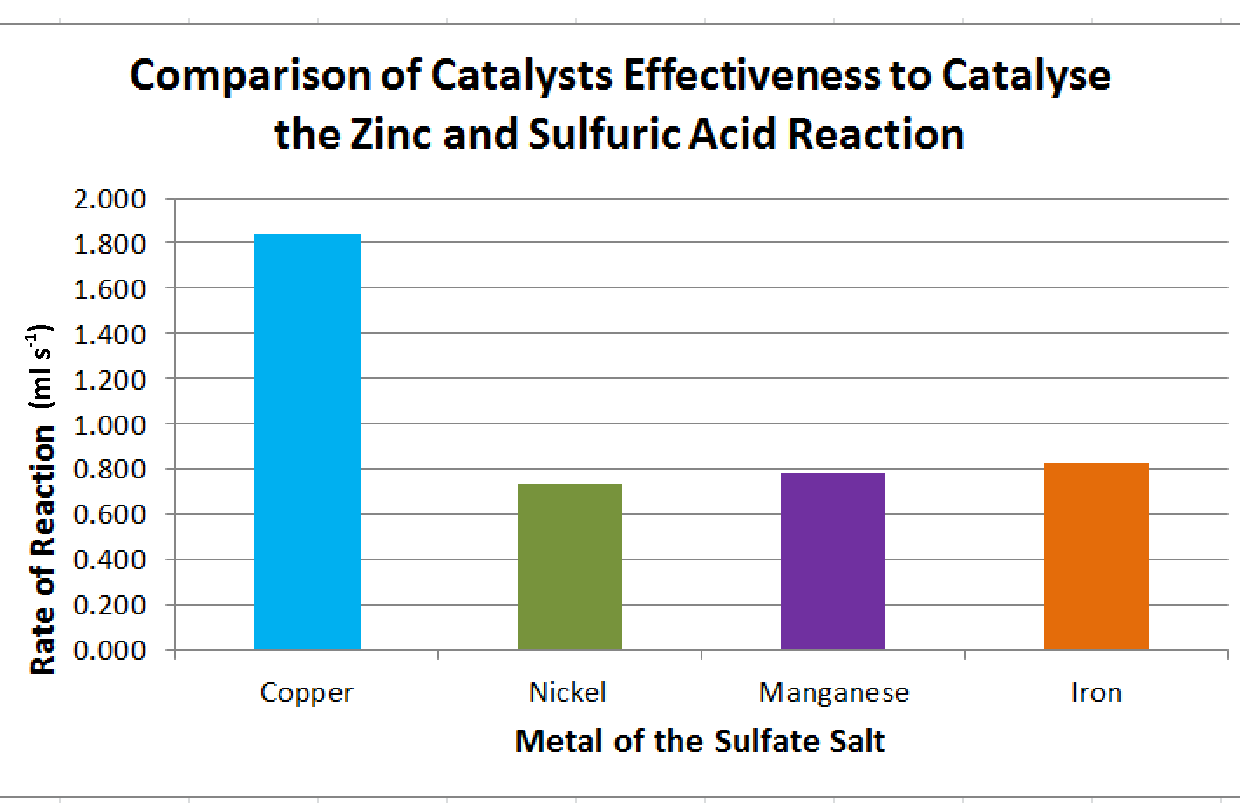
\includegraphics[width=\textwidth]{./Analysis/Images/4DifferentCatalysts/Comparison.pdf}
    \caption{Comparison of Rates of Different Sulfate Catalysts} \label{fig:ComparisonCat}
\end{figure}

This experiment has shown that copper sulfate is the most effective catalyst, which has over double the rate of all the other sulfates. Iron is the next most effective catalyst followed by manganese and then nickel.


\section{Investigating the Solubility of Hydrogen}

The graph below shows all of the data points taken from the raw data table in the Experiment section of my coursework. 

\begin{figure}[H]
    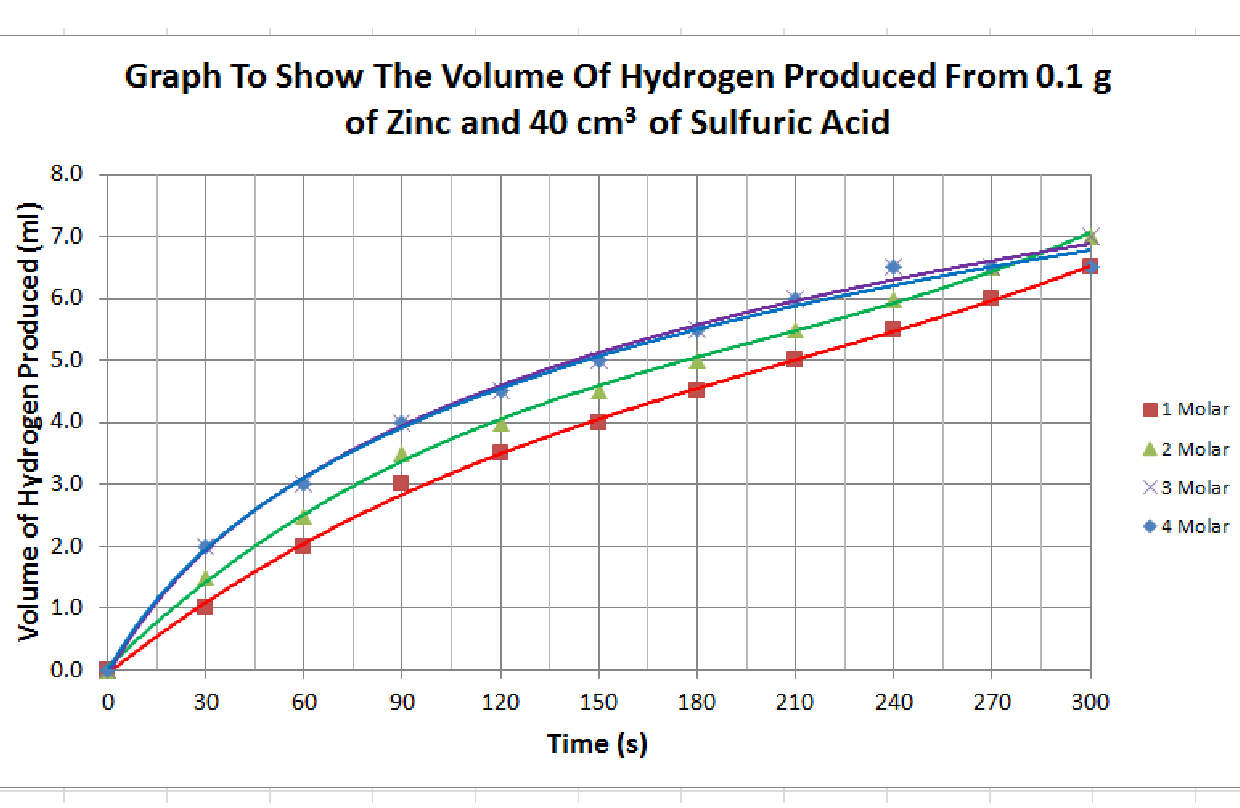
\includegraphics[width=\textwidth]{./Analysis/Images/Solubility.pdf}
    \caption{Comparison of the Hydrogen Produced When Different Concentrations of Sulfuric Acid is in Excess} \label{fig:ComparisonCat}
\end{figure}

Although there have been no scientific sources that I can find which discuss the solubility of hydrogen in higher concentrations of acids, my data starts to suggest that it does increase. At 4 molar sulfuric acid the volume of hydrogen produced is less than that of the lower concentrations which suggests that solubility of hydrogen does increase. To confidently comment on this, I would have to carry out the experiment with a wider range of acid concentrations. 